\documentclass[11pt, oneside]{article}
\usepackage[a4paper,bindingoffset=0.2in,%
            left=1in,right=1in,top=1in,bottom=1in,%
            footskip=.25in]{geometry}
\usepackage{graphicx}
\usepackage{enumerate}
\usepackage{url}
\usepackage{hyperref}
\usepackage{pbox}
\usepackage{CJKutf8}
\usepackage{mathtools}
\usepackage{microtype}
\usepackage[htt]{hyphenat}
\renewcommand{\vec}[1]{\mathbf{#1}}


\begin{document}
\title{Assignment 2: Practical PRML}
\author{Xiyou Zhou, 13307130189 \\ Computer Science and Technology}
\maketitle

\section{PCA for Feature Extraction, Visualization \& Classification}
First we can visualize the data in mnist dataset. We can see that each picture is a 28x28 square. What we need to do is to reduce the whole feature set of 784 to low-dimension feature space.
\begin{figure}[h]
\centering
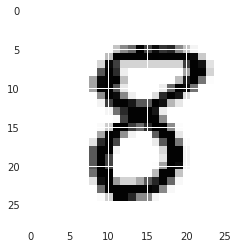
\includegraphics{./pics/mnist.png}
\caption{Plot of mnist data}
\end{figure}

The visualization of 2d and 3d plots with SVD and eigenvalue based approach are in the appendix.
The classification accuracy of KNN given neighbor number 3 are 95.23\%, 95.22\% and 93.38\% when feature space is reduced to 40, 80 and 200 dimensions with SVD-PCA approach. In order to preserve 95\% information or energy, we can use the percentage of total co-variance and use it to denote the information preserved, which was contained in pca.explained\_variance\_ratio\_. Therefore, the dimension is 334, which preserved 95.0\% information. The accuracy dropped to 88.85\%, probably due to overfit as the neighbor number is set as 3.

\section{LDA for Feature Extraction and Classification}
Visualizations can be found at appendix part. The test accuracy at dimension 2, 3 and 9 is 50.01\%, 71.19\% and 91.84\%. The maximum dimension that the data can be projected with LDA is 9, since eigenvalues are all 1 after this one, which means that the eigenvectors after 9 are just projections of manually added unit matrix.

\section{SVM for Classification}
Due to time reason, we only used 10\% of all training and test data here. We can see from the figures that accuracy jump from around 10\% to around 90\% when C changes from 0.01 to 10000 with different kernels. Meanwhile, larger C provides relatively better performance on accuracy. To radial kernels, larger dimension makes accuracy worse, which is reverse to linear kernel.Linear kernel has better overall performance while radial kernel's best performance is a little better. I think larger dimension provides linear kernel more information to process while radial kernel can be better fitted to dimension-reduced data.

\begin{figure}
\centering
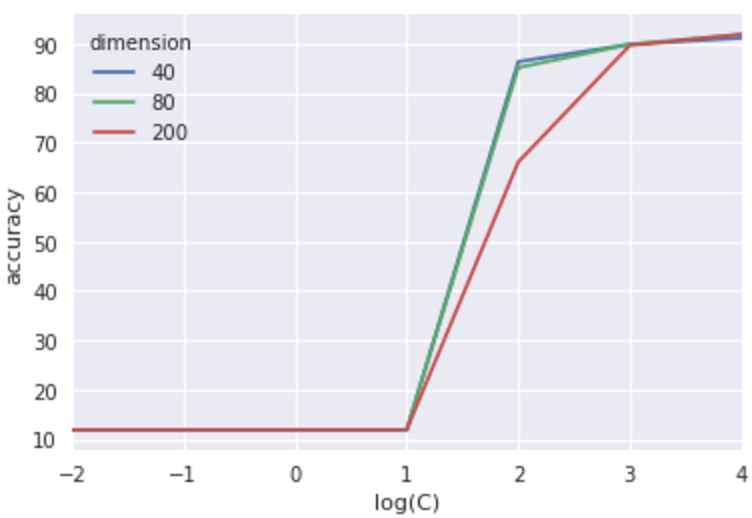
\includegraphics{./pics/radial_all.PNG}
\caption{Plot of SVM accuracy with radial kernel}
\end{figure}

\begin{figure}
\centering
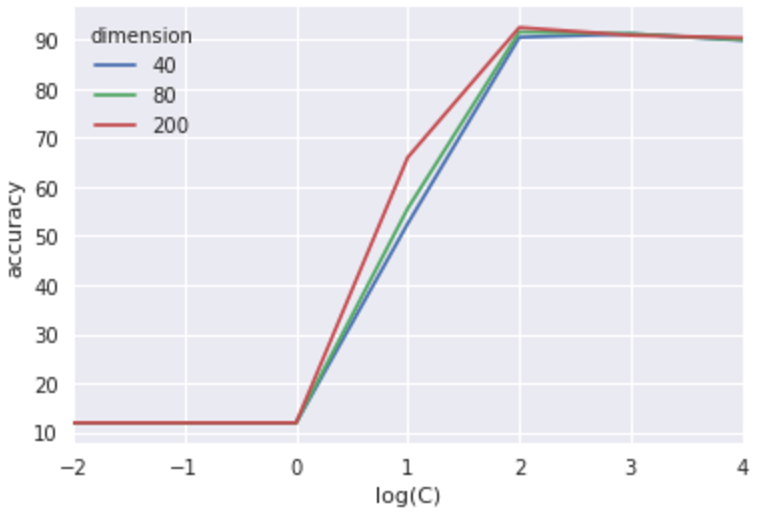
\includegraphics{./pics/linear_all.PNG}
\caption{Plot of SVM accuracy with linear kernel}
\end{figure}

\begin{figure}
\centering
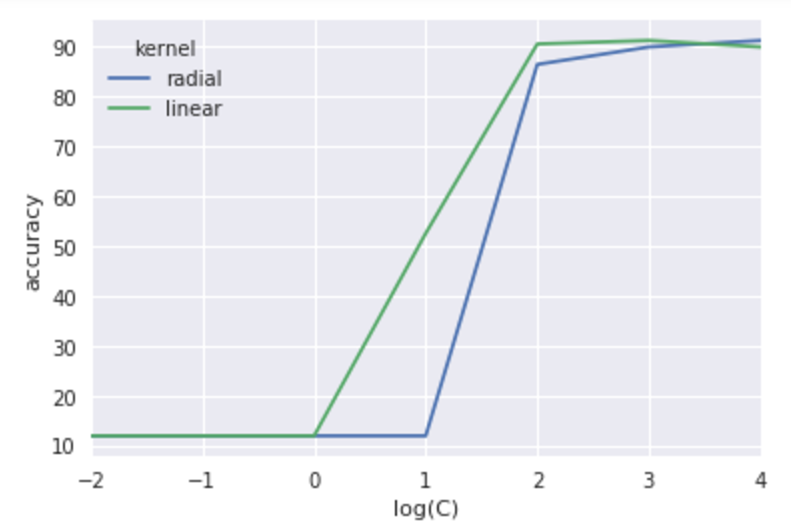
\includegraphics{./pics/d40.PNG}
\caption{Plot of SVM accuracy at dimension of 40 with different kernels}
\end{figure}

\begin{figure}
\centering
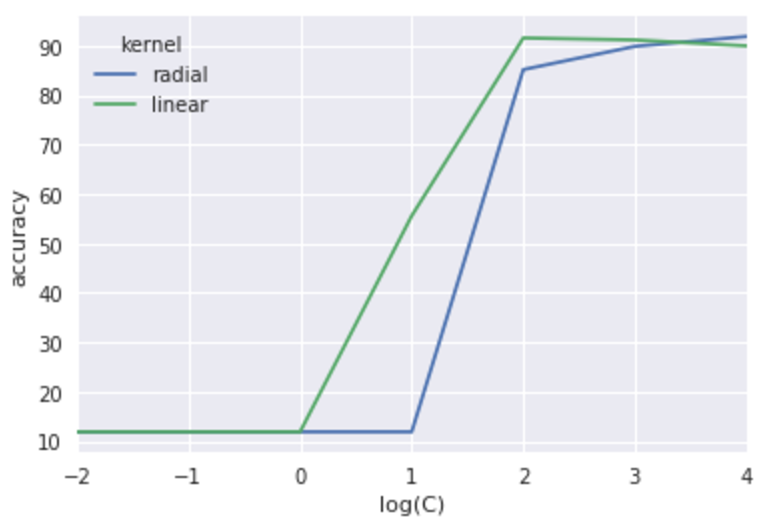
\includegraphics{./pics/d80.PNG}
\caption{Plot of SVM accuracy at dimension of 80 with different kernels}
\end{figure}

\begin{figure}
\centering
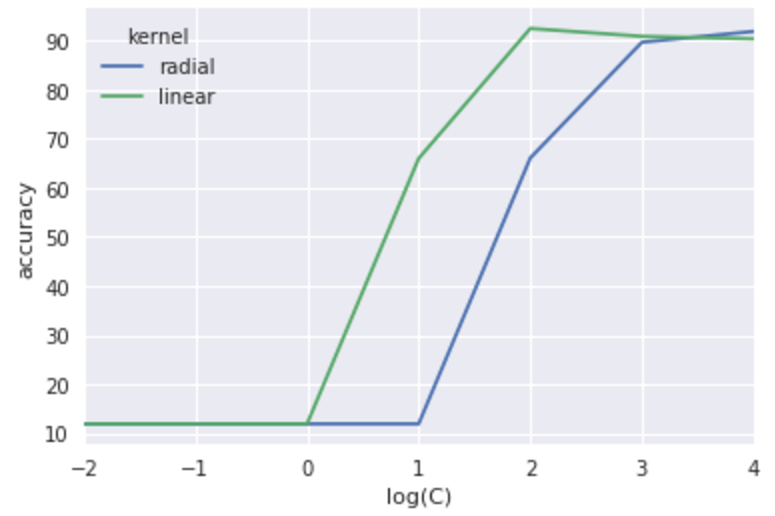
\includegraphics{./pics/d200.PNG}
\caption{Plot of SVM accuracy at dimension of 200 with different kernels}
\end{figure}

\section{Neural Network}
Deprecated.

\section{Survey}
12 hours in two days.


\begin{thebibliography}{9}
\bibitem{lucius-yu}
Implementing a Principal Component Analysis (PCA) in Python, step by step,
\\\texttt{http://sebastianraschka.com/Articles/2014\_pca\_step\_by\_step.html}

\bibitem{princeton}
A Tutorial on Principal Component Analysis,
\\\texttt{https://www.cs.princeton.edu/picasso/mats/PCA-Tutorial-Intuition\_jp.pdf}

\bibitem{test}
Linear Discriminant Analysis Bit by Bit,\\
\texttt{http://sebastianraschka.com/Articles/2014\_python\_lda.html}

\end{thebibliography}

\section{Appendix}
Please see the plots below attached.

\begin{figure}[h]
\centering
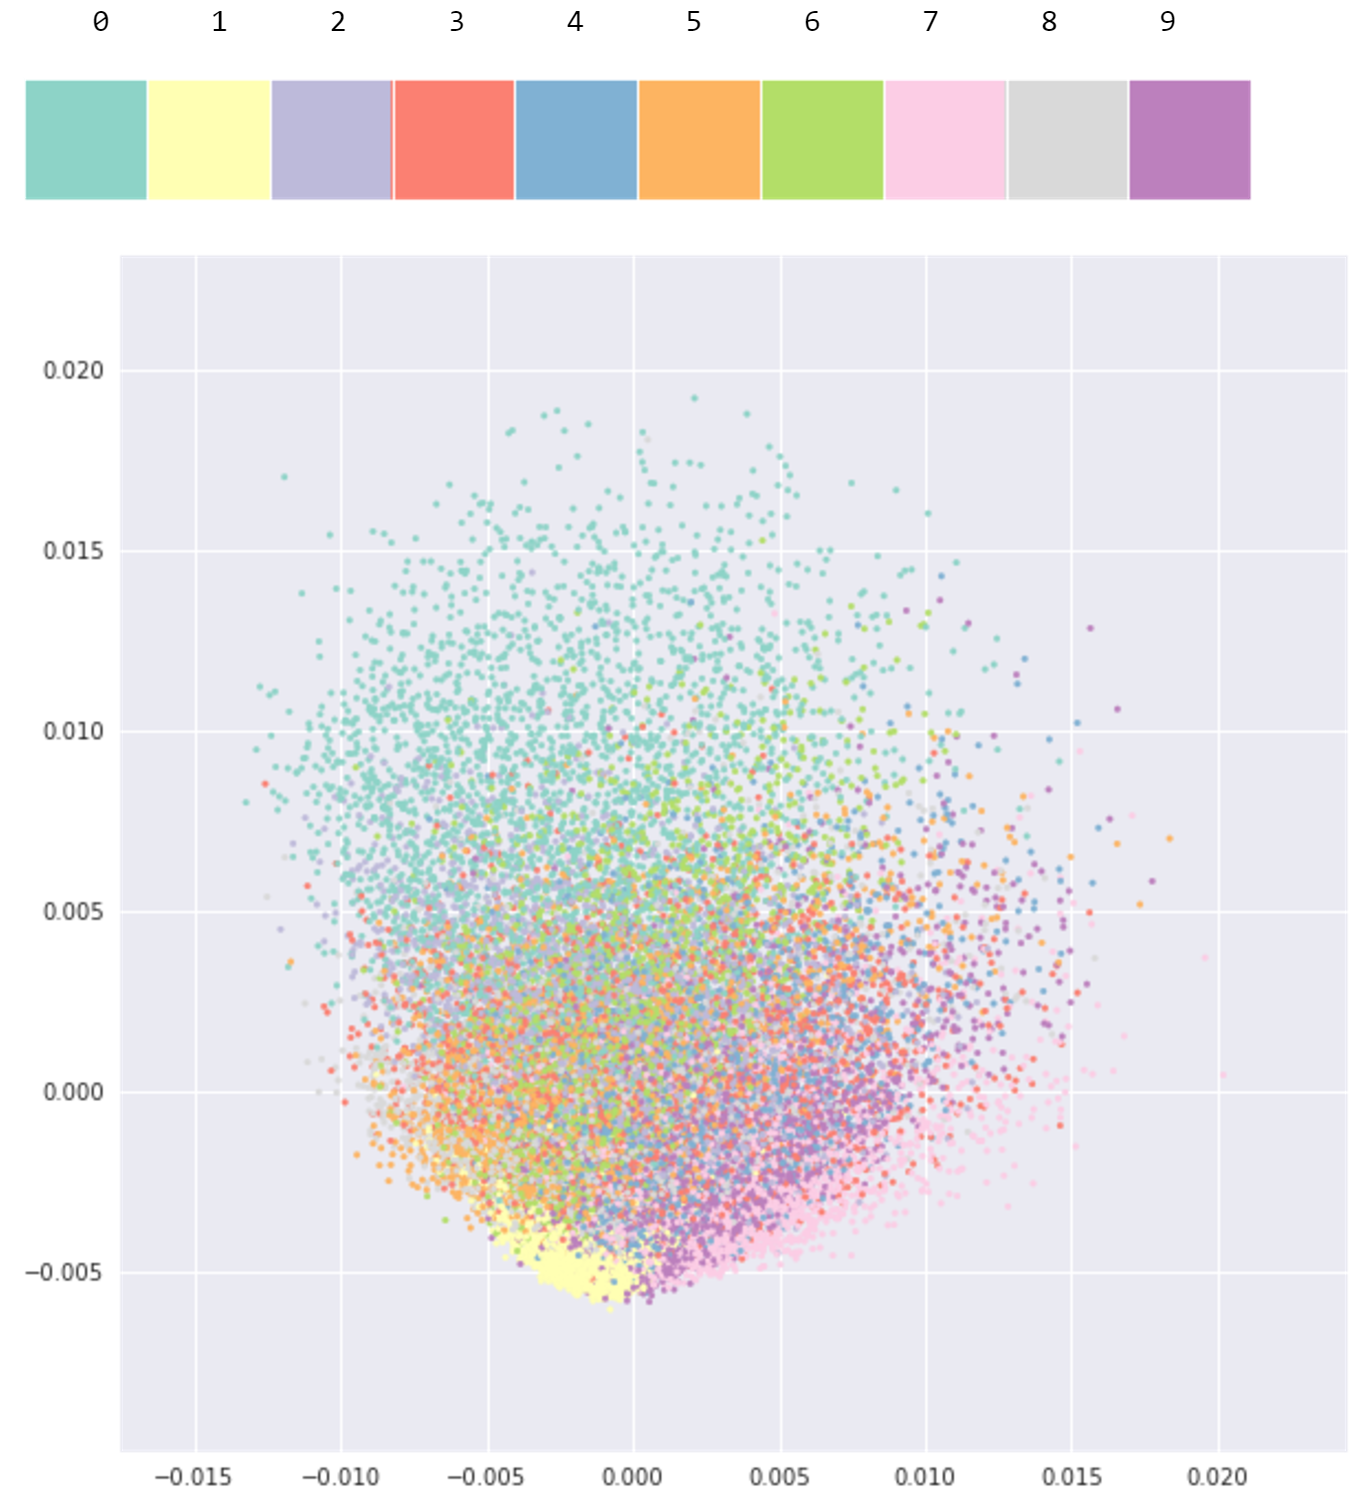
\includegraphics{./pics/svd_pca_2d.PNG}
\caption{Plot of SVD based PCA 2d visualization}
\end{figure}

\begin{figure}[h]
\centering
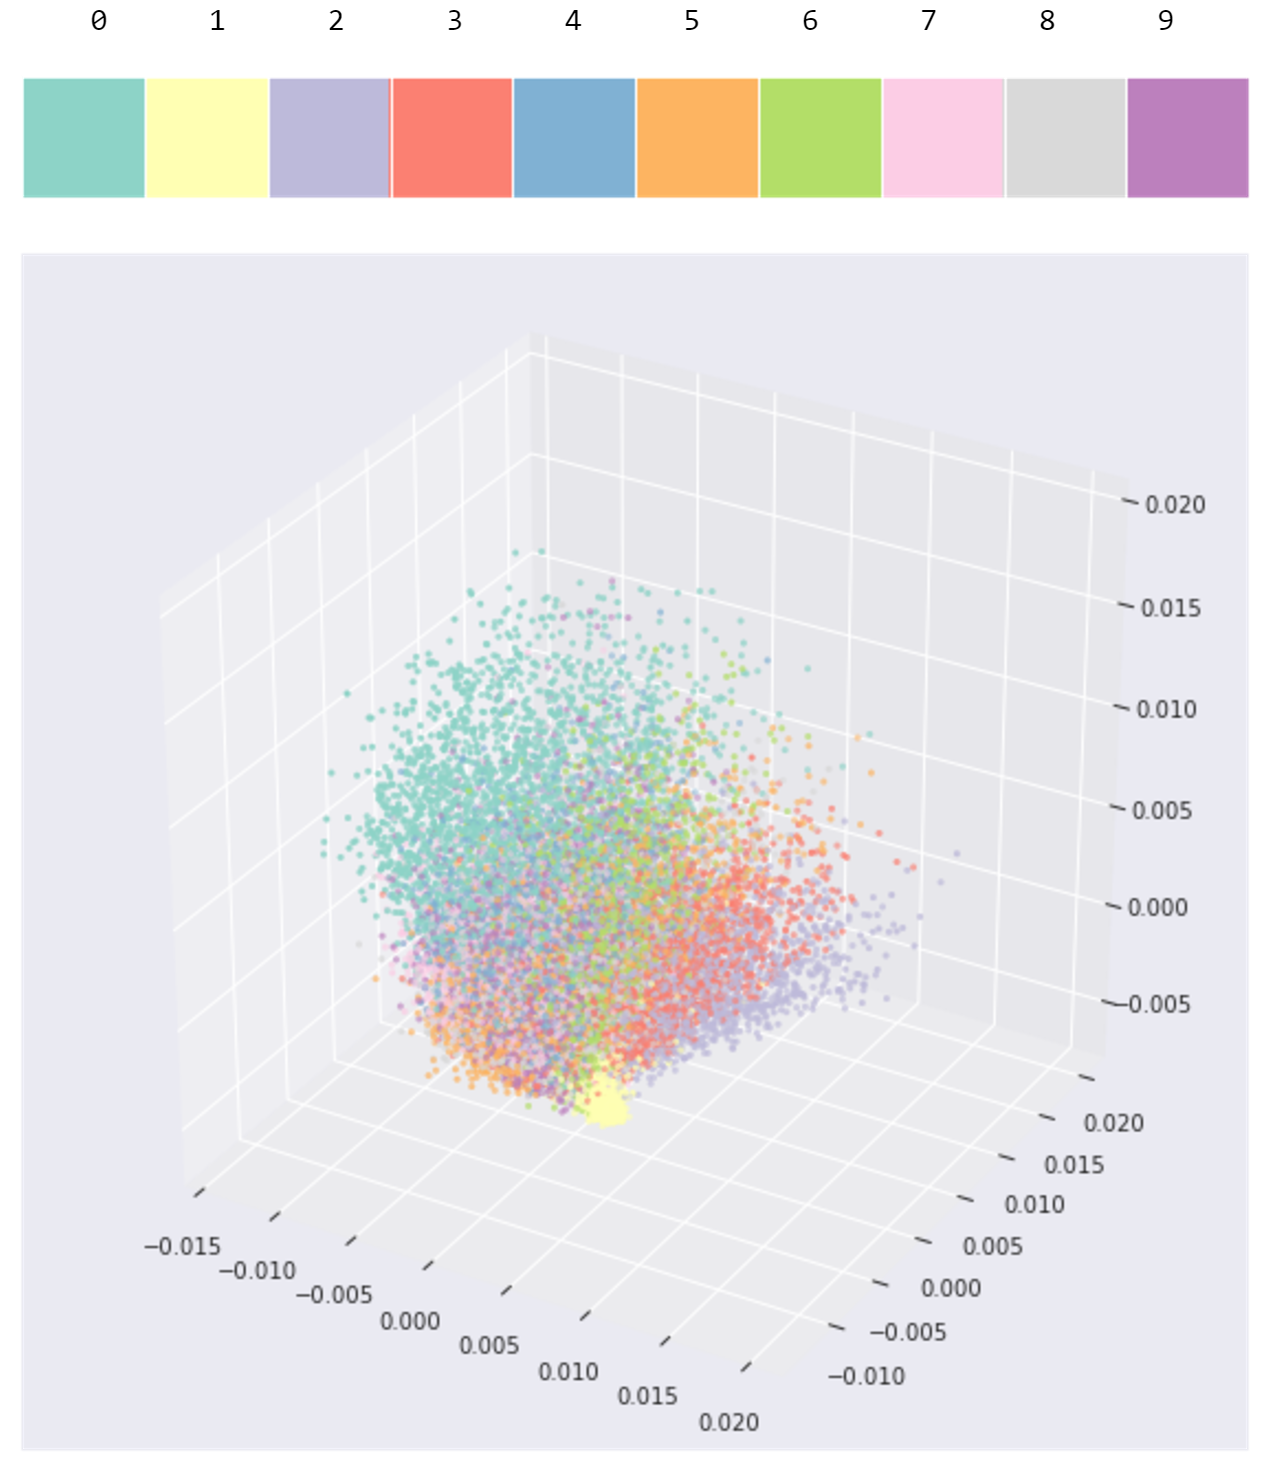
\includegraphics{./pics/svd_pca_3d.PNG}
\caption{Plot of SVD based PCA 3d visualization}
\end{figure}

\begin{figure}[h]
\centering
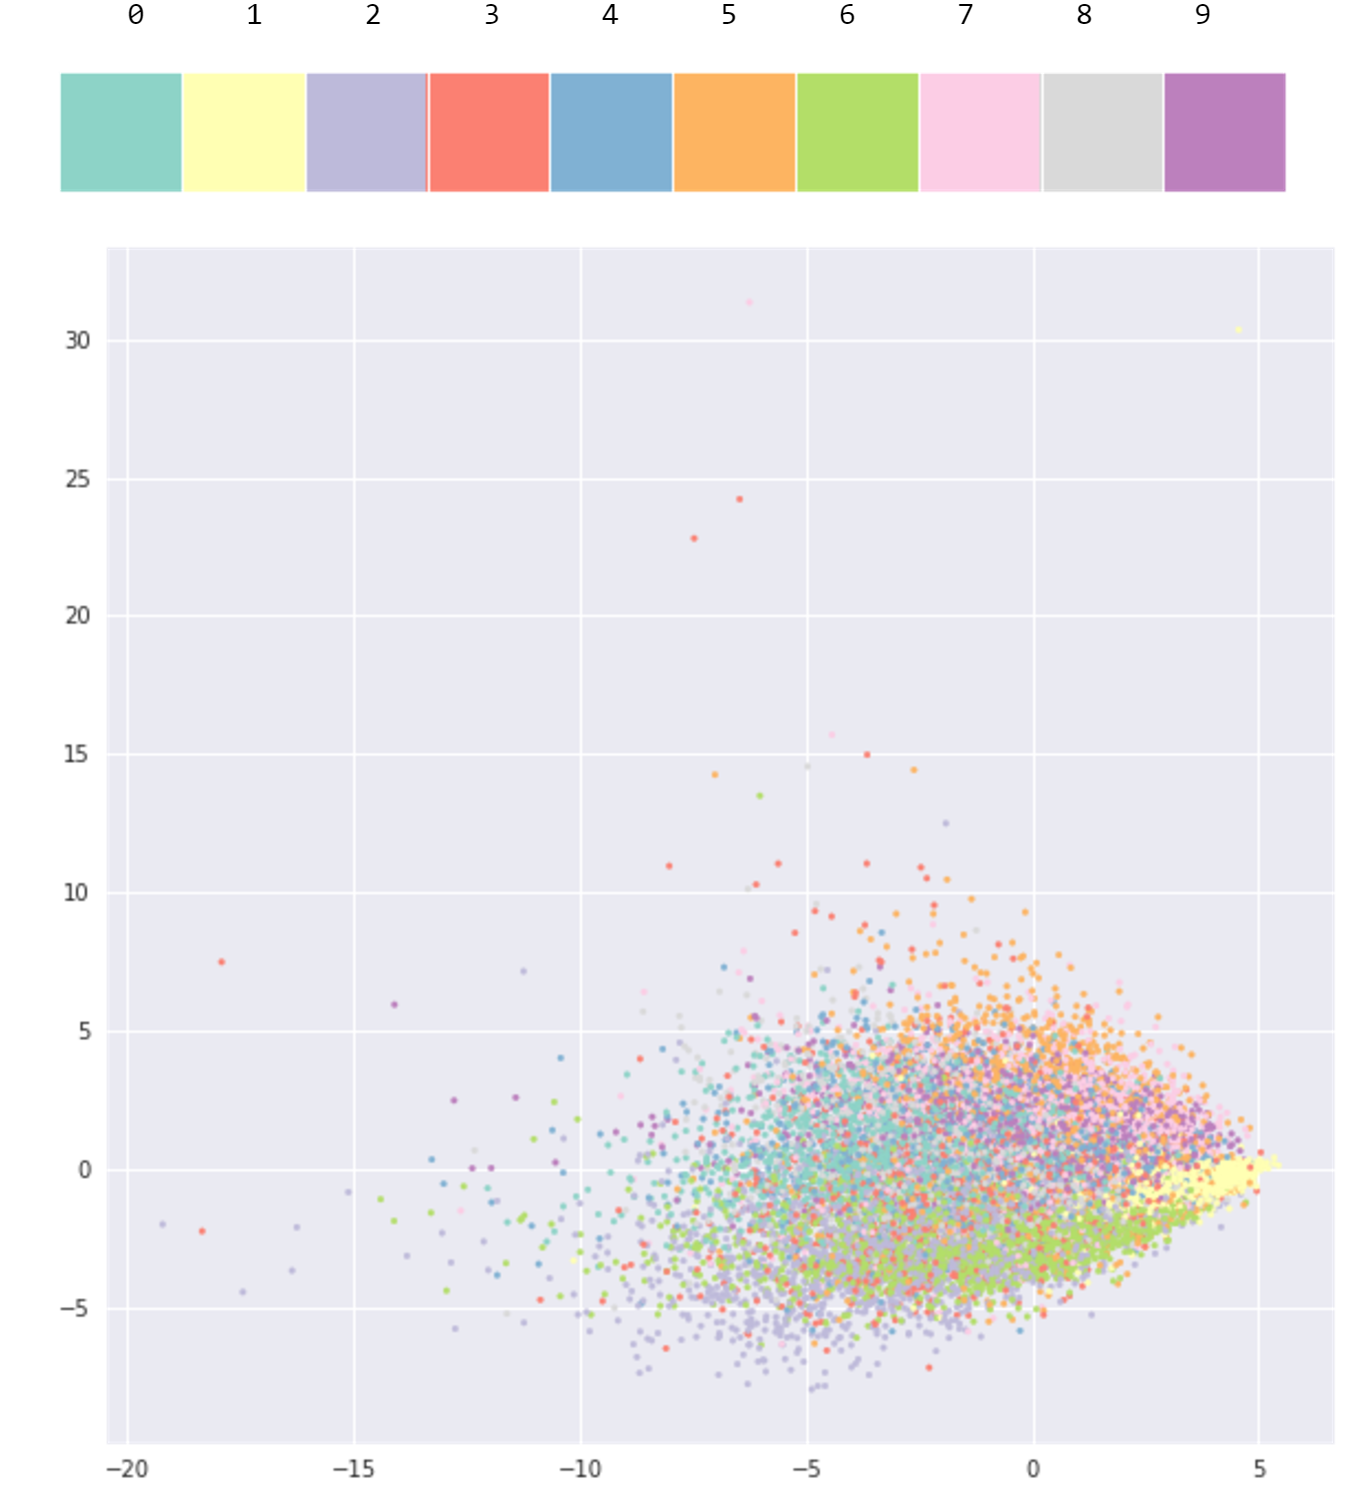
\includegraphics{./pics/cov_pca_2d.PNG}
\caption{Plot of Eigenvalue based PCA 2d visualization}
\end{figure}

\begin{figure}[h]
\centering
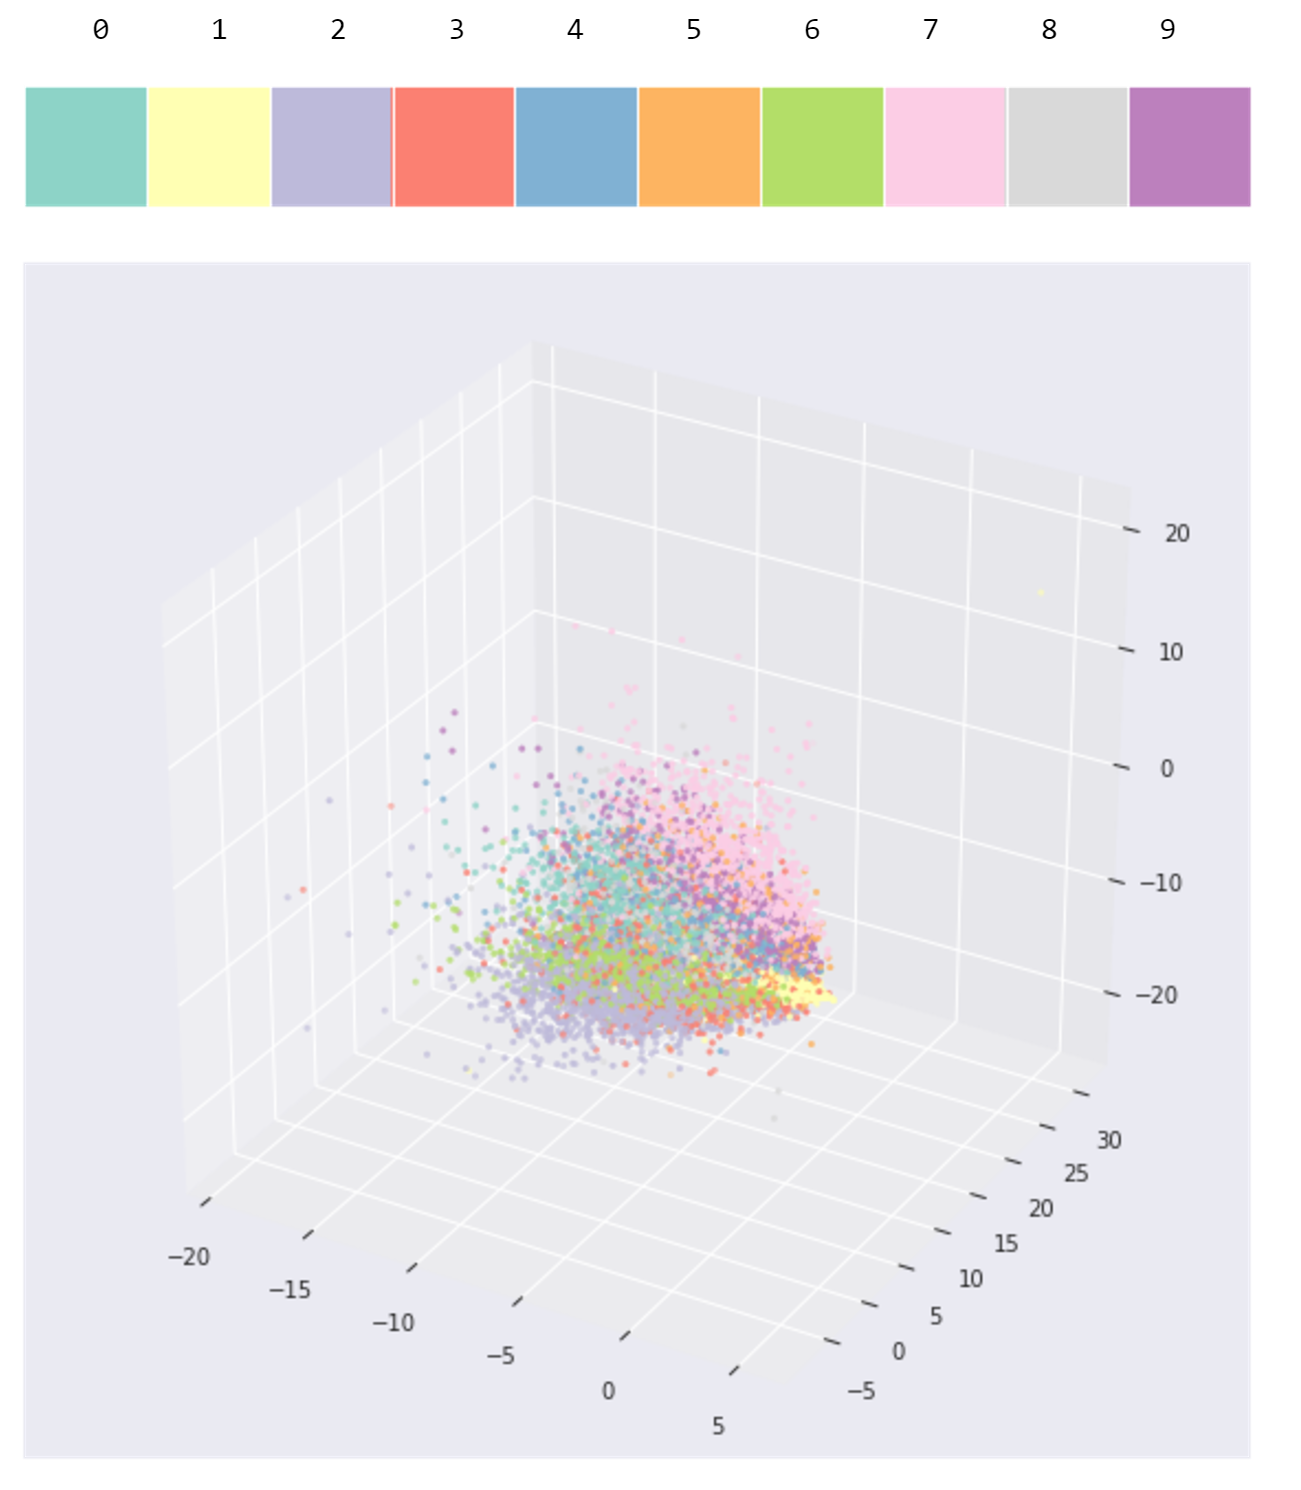
\includegraphics{./pics/cov_pca_3d.PNG}
\caption{Plot of Eigenvalue based PCA 3d visualization}
\end{figure}

\begin{figure}[h]
\centering
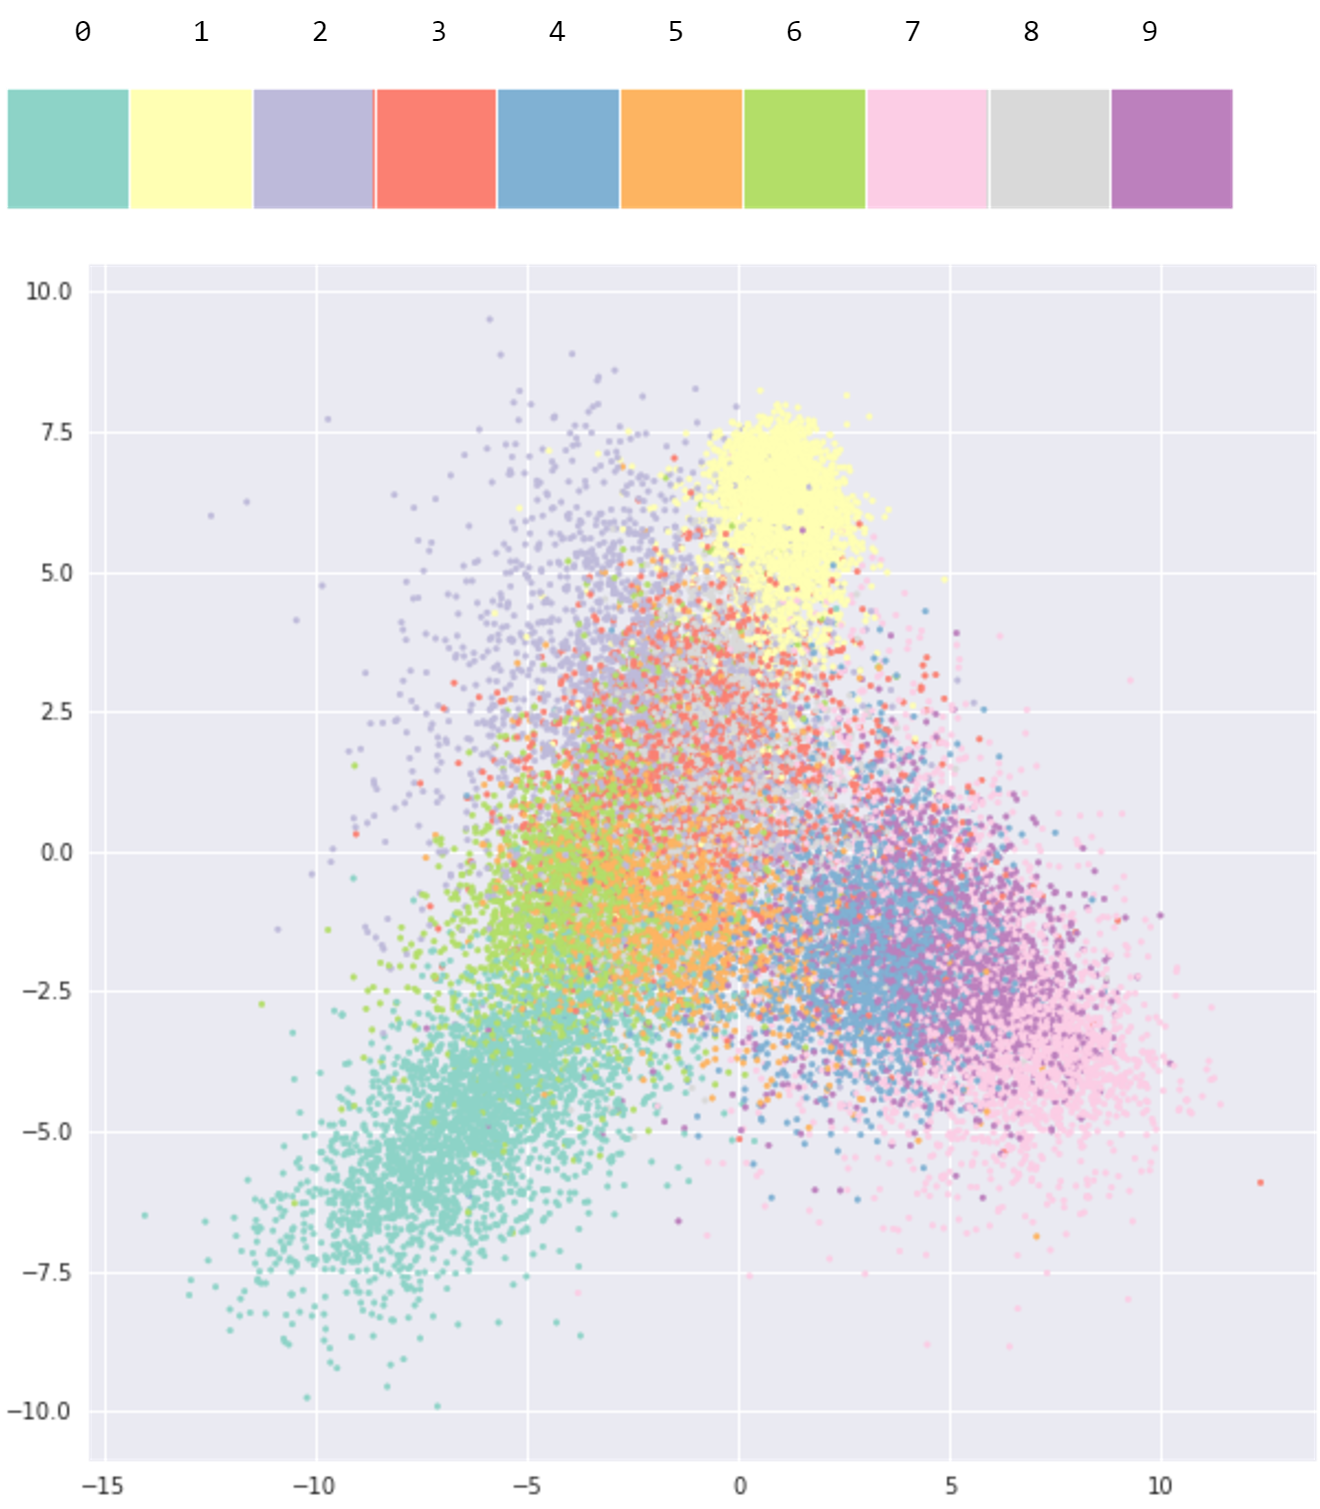
\includegraphics{./pics/cov_lda_2d.PNG}
\caption{Plot of LDA feature extraction 2d visualization}
\end{figure}

\begin{figure}[h]
\centering
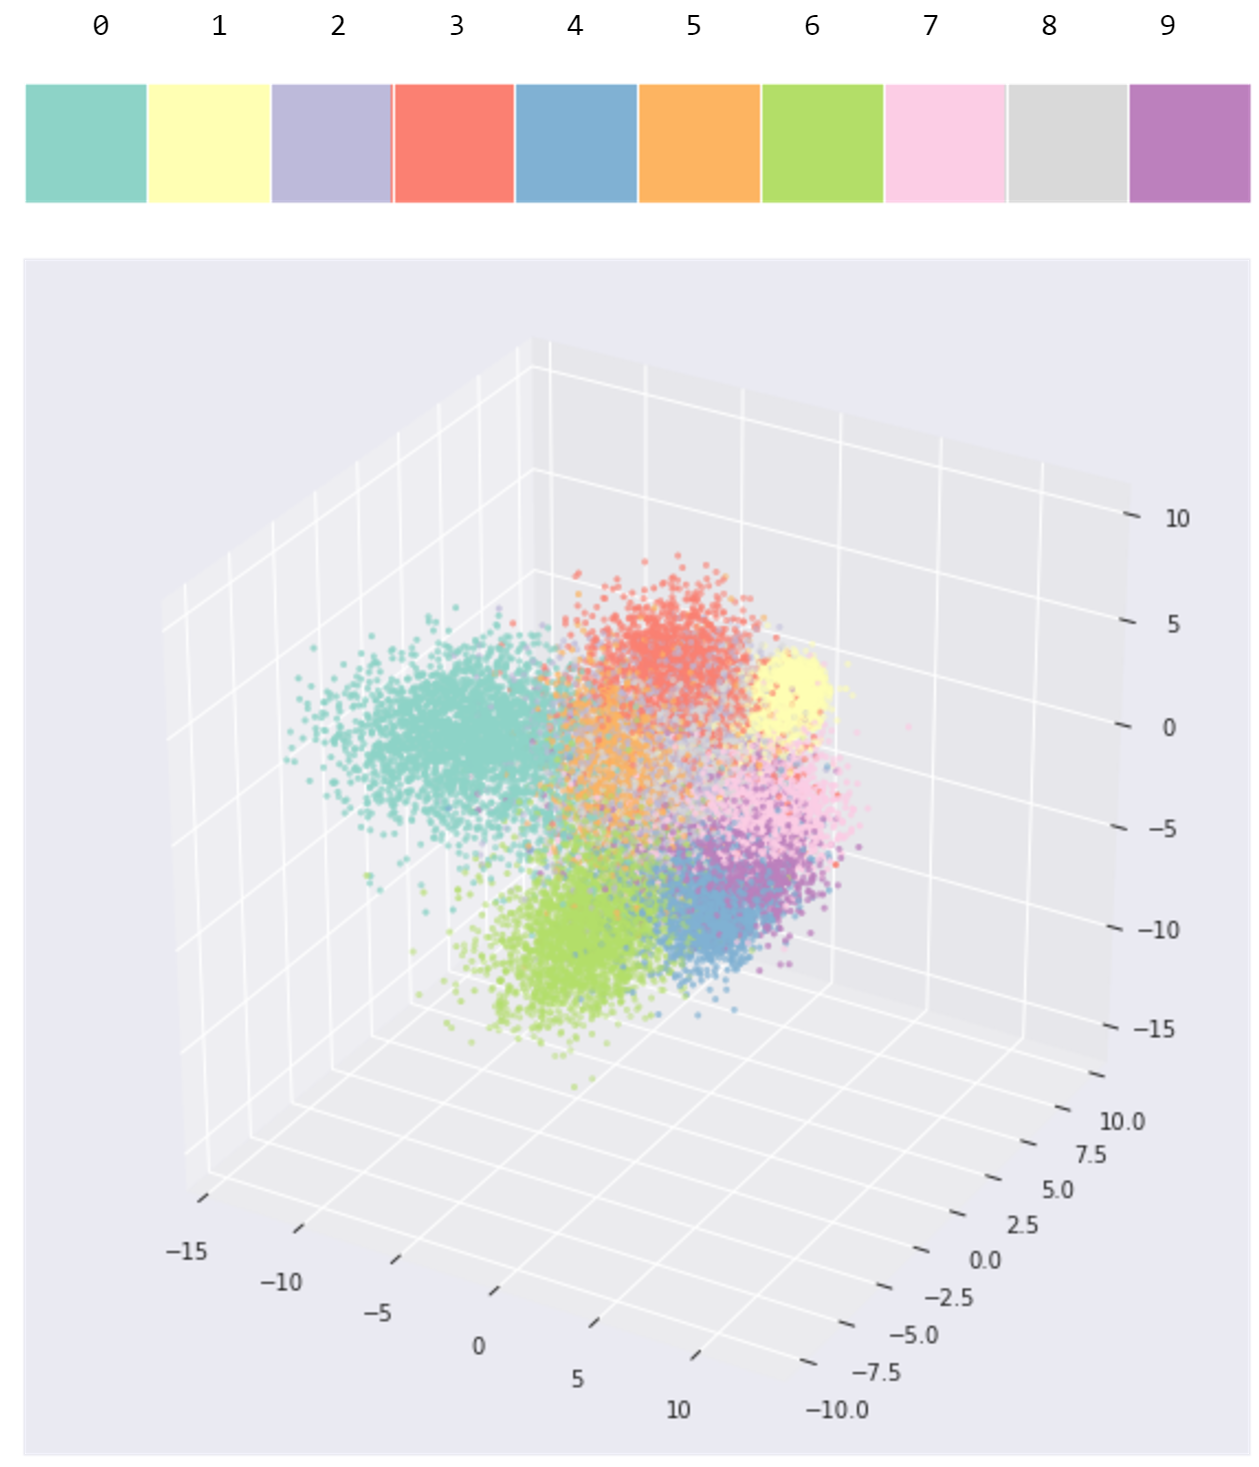
\includegraphics{./pics/cov_lda_3d.PNG}
\caption{Plot of LDA feature extraction 3d visualization}
\end{figure}

\begin{figure}
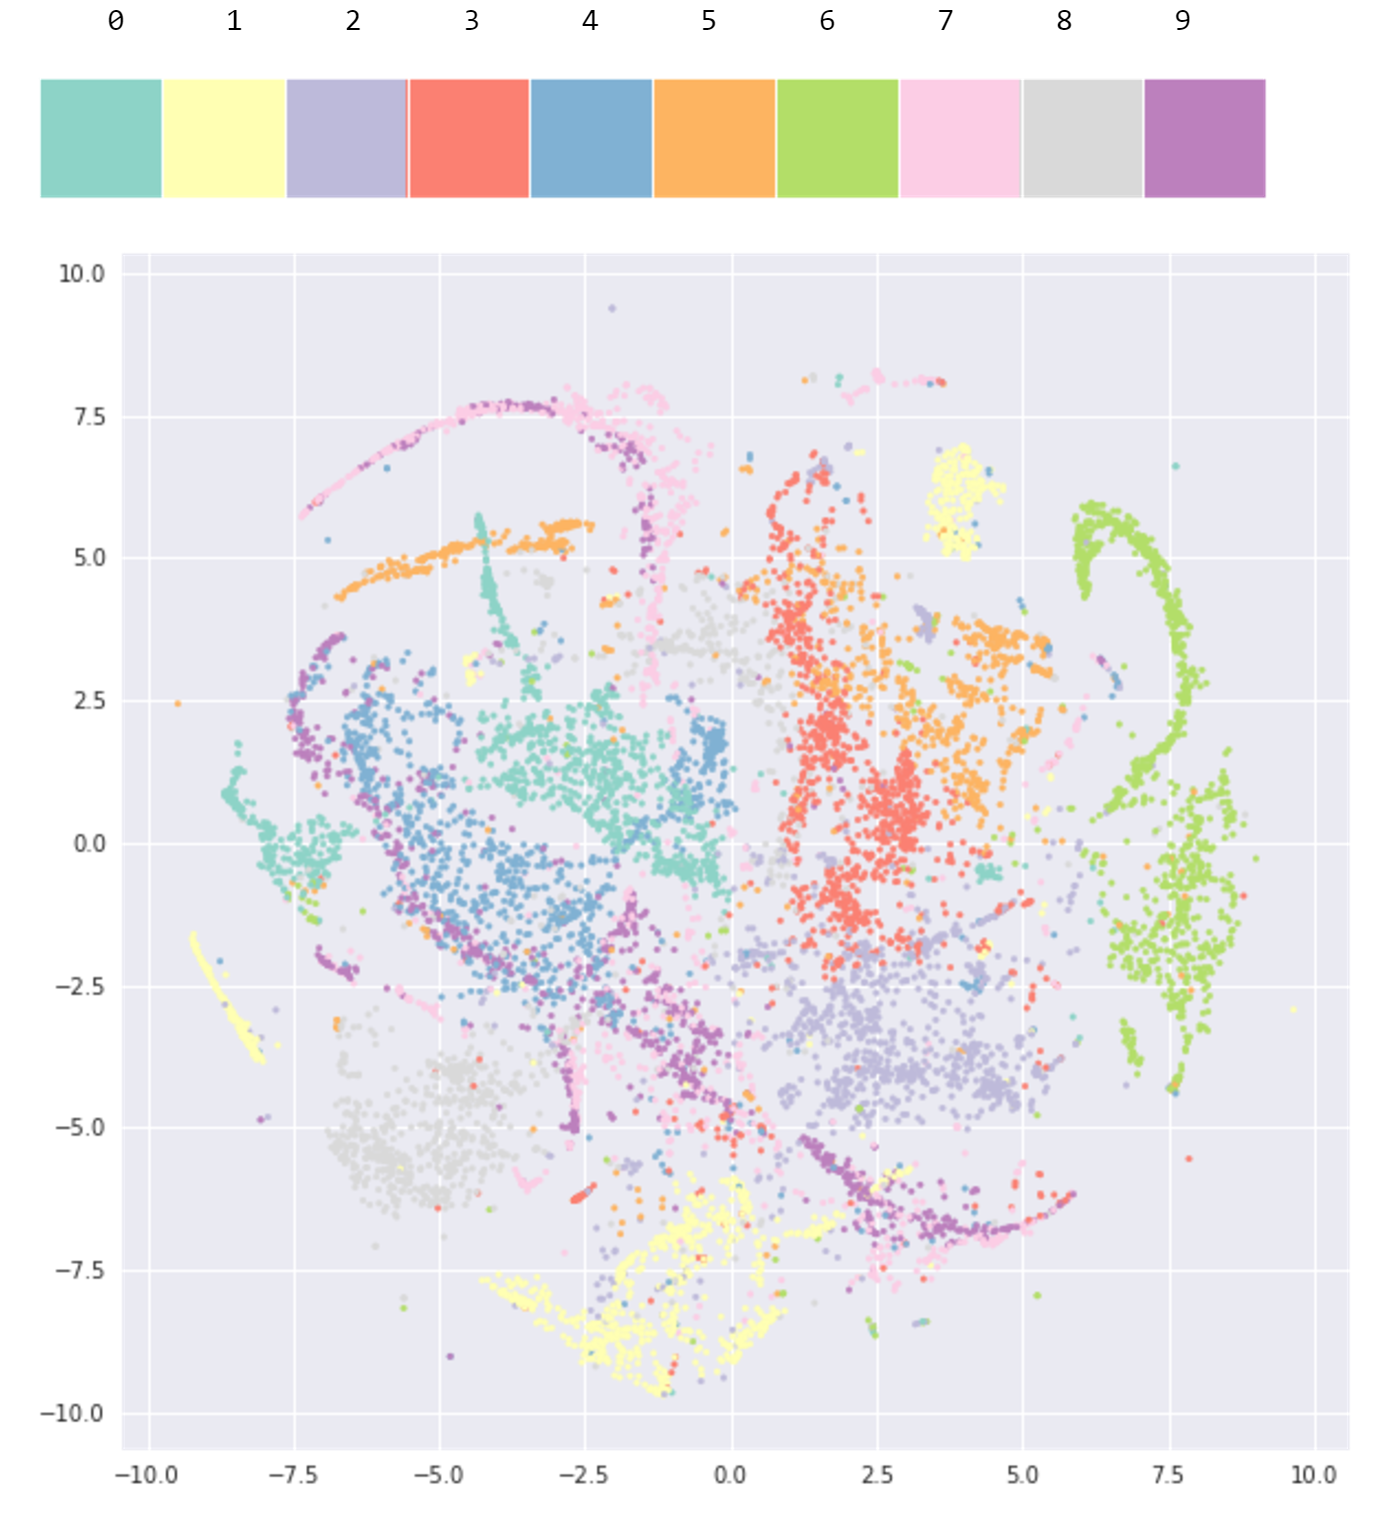
\includegraphics{./pics/tsne_pca_2d.PNG}
\caption{Plot of t-SNE 2d visualization of mnist dataset}
\end{figure}

\begin{figure}
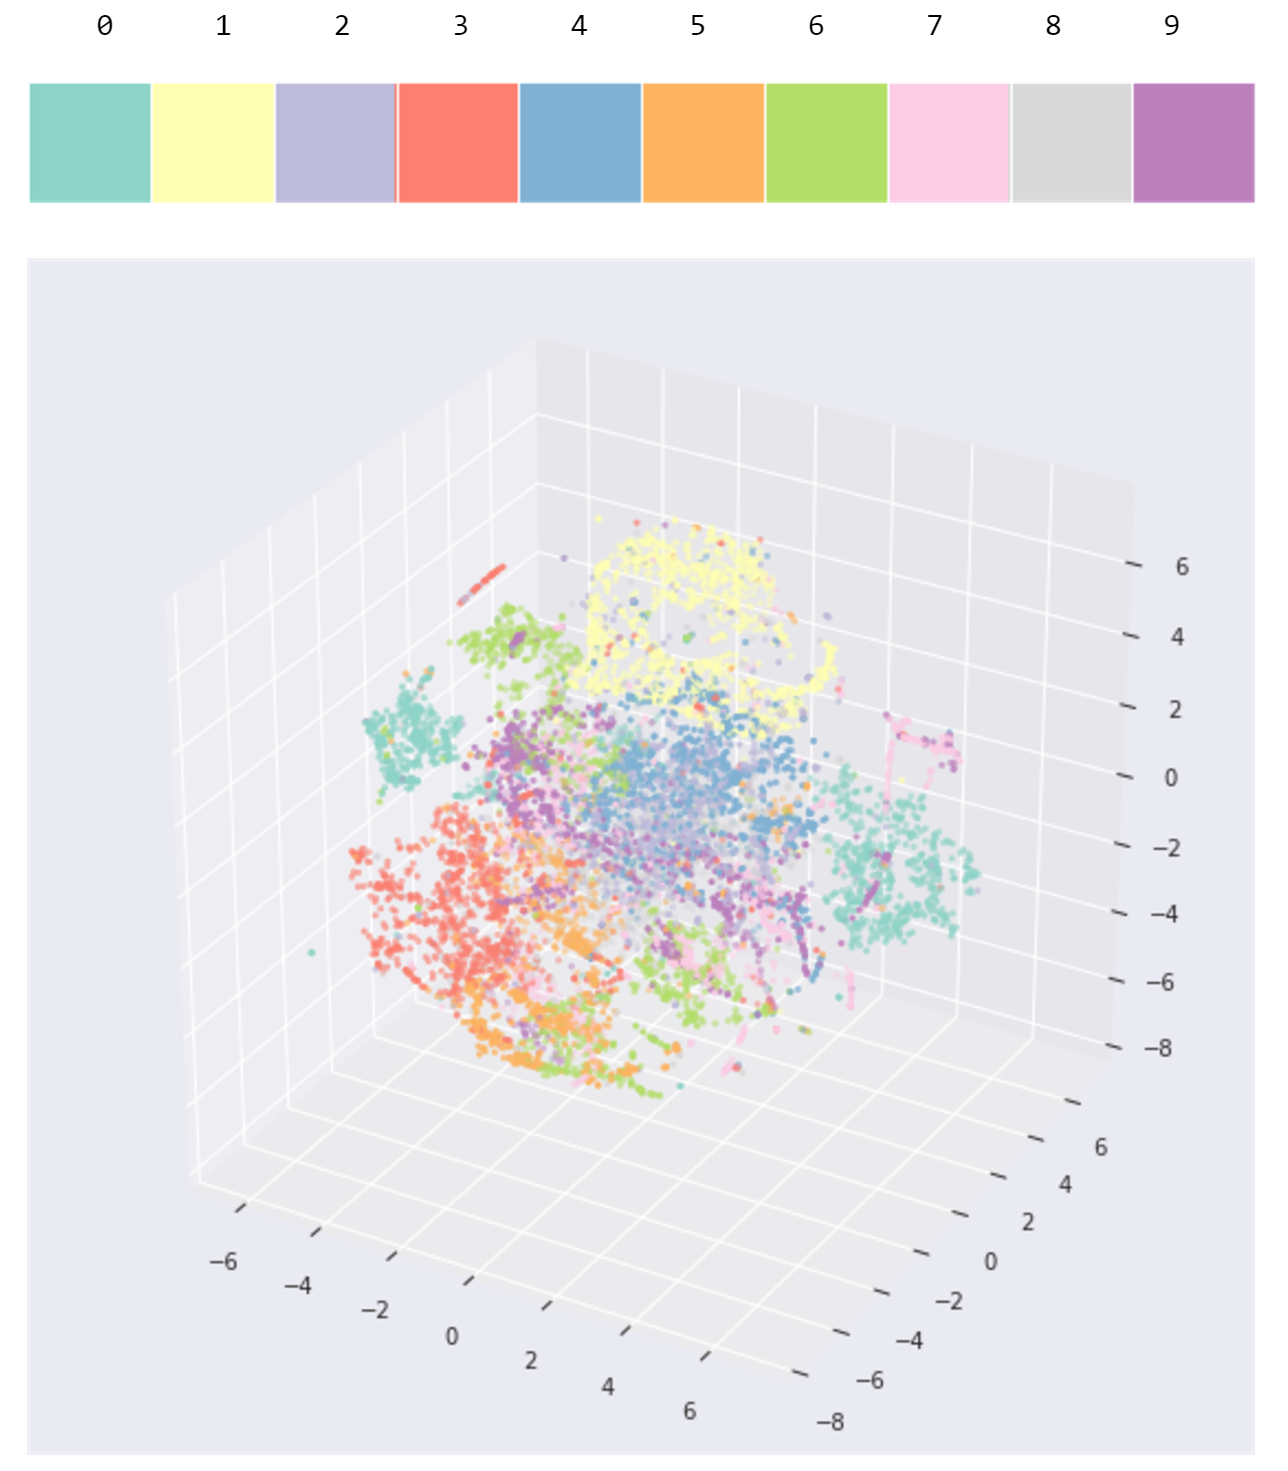
\includegraphics{./pics/tsne_pca_3d.PNG}
\caption{Plot of t-SNE 3d visualization of mnist dataset}
\end{figure}

\end{document}